% Template for Cogsci submission with R Markdown

% Stuff changed from original Markdown PLOS Template
\documentclass[10pt, letterpaper]{article}

\usepackage{cogsci}
\usepackage{pslatex}
\usepackage{float}
\usepackage{caption}

% amsmath package, useful for mathematical formulas
\usepackage{amsmath}

% amssymb package, useful for mathematical symbols
\usepackage{amssymb}

% hyperref package, useful for hyperlinks
\usepackage{hyperref}

% graphicx package, useful for including eps and pdf graphics
% include graphics with the command \includegraphics
\usepackage{graphicx}

% Sweave(-like)
\usepackage{fancyvrb}
\DefineVerbatimEnvironment{Sinput}{Verbatim}{fontshape=sl}
\DefineVerbatimEnvironment{Soutput}{Verbatim}{}
\DefineVerbatimEnvironment{Scode}{Verbatim}{fontshape=sl}
\newenvironment{Schunk}{}{}
\DefineVerbatimEnvironment{Code}{Verbatim}{}
\DefineVerbatimEnvironment{CodeInput}{Verbatim}{fontshape=sl}
\DefineVerbatimEnvironment{CodeOutput}{Verbatim}{}
\newenvironment{CodeChunk}{}{}

% cite package, to clean up citations in the main text. Do not remove.
\usepackage{apacite}

% KM added 1/4/18 to allow control of blind submission


\usepackage{color}

% Use doublespacing - comment out for single spacing
%\usepackage{setspace}
%\doublespacing


% % Text layout
% \topmargin 0.0cm
% \oddsidemargin 0.5cm
% \evensidemargin 0.5cm
% \textwidth 16cm
% \textheight 21cm

\title{Children's understanding of simple polite markers}


\author{{\large \bf } \\ \texttt{} \\  \\}

\begin{document}

\maketitle

\begin{abstract}
What do children understand about polite speech? Here we show that, with
an improvement over the age of 2 to 4 years, English-speaking preschool
children understand implications of simple polite markers: They
understand that it is more polite and nicer (and less rude and mean) to
use polite markers such as ``please'' when making requests, and that the
use of these polite markers indicates that the speaker is more socially
likeable and is more likely to gain compliance from their conversational
partners. This work can help lay the foundation for future work on
children's understanding of polite speech.

\textbf{Keywords:}
Politeness, pragmatic development, online experiment
\end{abstract}

\section{Introduction}\label{introduction}

We use and hear polite speech on a daily basis: polite utterances range
from simple words of apology (``sorry'') or gratitude (``thanks'') to
compliments (``I love your dress!'') to ways of making requests (``Can
you please open the window?''). Yet polite utterances are seemingly
inefficient and even misinformative: speakers say ``Can you
please\textasciitilde{}'' when it should suffice to say, ``Open the
window.'' This creates a mystery for classical views of language as
information transfer (Buhler, 1934; Goodman \& Stuhlmuller, 2013;
Jakobson, 1960; Shannon, 1948): If language is a tool for transferring
information, speakers should be as efficient as possible in their
communication to prioritize informativity. Nonetheless, speakers use
politeness strategies often, even while arguing (Holtgraves, 1997),
though polite language (indirect speech or white lies) may lead to
misunderstandings (Bonnefon, Feeney, \& De Neys, 2011).

So why do people speak politely? Linguistic theories assume that
people's utterance choices are motivated by social concerns, framed as
either maxims (Leech, 1983), social norms (Ide, 1989), or listener's
and/or speaker's public identity (\emph{face}; Brown \& Levinson, 1987).
For example, Brown \& Levinson (1987)'s theory predicts that a speaker's
intended meaning contains a threat to the listener's face or self-image,
the speaker's utterance will be less direct and informative. Thus,
because saying ``open the window'' might give an impression that the
speaker assumes she is in a position to give orders to the listener, she
would say instead, ``Can you please open the window?'' since conveying
the message in a more indirect form of request gives the other person a
sense of autonomy or freedom from imposition (Clark \& Schunk, 1980).
Thus, while it may hinder the goals of efficient information transfer,
using polite speech can help the listener save his face and feel good
about himself, while inferring that the speaker had kind motives as well
(Yoon, Tessler, Goodman, \& Frank, 2017).

Do children speak politely, and if so what do they understand about
polite speech? Children begin producing polite speech early on; They
start producing the simple polite marker ``please'' at 2.5 years (Read
\& Cherry, 1978), and request forms increase in their variety and
frequency with age (Bates, 1976; Bates \& Silvern, 1977; Bock \&
Hornsby, 1981; Ervin-Tripp, 1982; Nippold, Leonard, \& Anastopoulos,
1982). Young children learn to produce different forms of requests
depending on context: For example, by three years children are able to
vary their utterances based on whether they are instructed to ``tell''
versus ``ask'' an addressee to given them a puzzle piece (Bock \&
Hornsby, 1981). By two years, children are able to modify their requests
to make them more polite (``ask in the nicest way possible''; Bates \&
Silvern, 1977). Hence children's \emph{production} of polite speech
seems to parallel adult speakers' desires to produce utterances with
appropriate levels of face-saving.

Evidence for children's \emph{comprehension} of polite speech, on the
other hand, is much sparser compared to production, and have been
largely inconclusive. For example, upon hearing someone making a request
(``Please pour me more water''), how might children evaluate this
speaker? Though there was some initial evidence to suggest that
producing a request with ``please'' is judged to be polite by three
years of age (Bates, 1976; Bates \& Silvern, 1977), in a later study,
the judgment of ``please'' as being polite was only replicated starting
at five years of age, but not younger (Nippold et al., 1982). These
initial studies also have additional unresolved issues, including the
lack of statistical tests to assess each age group's performance, and
lack of systematic manipulation of cues other than linguistic markers
(e.g., prosody or facial expressions).

Thus, there are many open questions about children's understanding of a
speaker's intentions behind polite speech. For example, do children know
the word ``polite'' should be associated with politeness rules people
abide by (e.g., saying ``please'')? Relatedly, do children recognize
polite speech as being positively valenced, such that they think it is
better and nicer to say polite things? Also, do children understand
social implications of speaking politely, such that people who are
polite may be more likely to get their wishes granted (``I will pour him
more water because he was nice'') and may be better social partners
compared to those who are impolite. Finally, what cues to politeness do
children recognize? Do they recognize linguistic markers such as
``please,'' or ``can you,'' or both? Or do they rely on prosodic cues
that make utterances sound more respectful, or on facial expressions
that make a person look kind?

In this current work, we sought to answer these questions, and test what
2- to 4-year-old children understand about polite speech. Across three
Experiments, we presented stories about speakers who decided to speak
politely (e.g., ``Please pour me more water'') or impolitely (e.g.,
``Pour me more water'') and asked child participants to compare between
the two speakers. We were interested to know if children were sensitive
to a speaker's use of simple polite markers (e.g., ``please'') and
examined whether: (1) children are able to reason about speakers using
polite speech as being ``polite'' and ``nice'' and not ``rude'' or
``mean''; (2) they can reason about social implications of using polite
speech (e.g., politeness as a sign of a nice play partner) (3) they show
improvement with age for these lines of reasoning (4) they have to rely
on other additional cues such as facial expressions (Expt 1) or prosodic
cues (Expt 2), or they can make use of linguistic markers alone (Expt 3)
to make appropriate inferences about the speaker.

\section{Experiment 1}\label{experiment-1}

In Experiment 1, we tested whether 3- to 4-year-old children were able
to understand implications of using simple polite markers, based on not
only linguistic cues of interest (whether the speaker says ``please,''
``can you''), but also extra cues that they might need (facial
expressions and prosodic cues). Thus, we asked children to compare
between speakers who used polite markers with a kind voice and facial
expression versus speakers who did not use polite markers and spoke with
a mean, angry voice and facial expression.

\subsection{Methods}\label{methods}

\subsubsection{Participants}\label{participants}

3-year-old (\(n=\) 20; 12 F, \(M_{age}\) = 3.61 years, \(SD_{age}\) =
0.22) and 4-year-old children (\(n=\) 18; 6 F, \(M_{age}\) = 4.38 years,
\(SD_{age}\) = 0.25) were recruited from a local preschool. An
additional 3 children were tested but excluded due to failure on the
practice questions (\(n=\) 2) or completion of fewer than half of the
test trials (\(n=\) 1).

\subsubsection{Stimuli and design}\label{stimuli-and-design}

We designed a picture book with twelve stories in which a protagonist is
approached by two speakers, one of whom makes a request by producing an
utterance with a polite marker (e.g., ``Please pour me more water''),
and the other produces an utterance without (``Pour me more water'').
There were three types of polite marker that could be used: ``please''
(as in ``Please pour me more water''), ``can you'' (``Can you pour me
more water''), and ``can you please'' (``Can you please pour me more
water'').

We designed six question types to ask participants following the
presentation of the stories: four \emph{speaker attribute} questions
(\emph{polite}: ``Which one was more polite?''; \emph{rude}: ``Which one
was more rude?''; \emph{nice}: ``Which one was nicer?''; \emph{mean}:
``Which one was meaner?'') and two \emph{social implication} questions
(\emph{play partner}: ``Which one would you rather play with?'';
\emph{compliance}: ``Which one will {[}get what they want{]}?''). Each
participant would be asked one of the four speaker attribute questions,
followed by one of the two social implication questions.

In Experiment 1, all utterances were produced live by the experimeter,
with appropriate proodic cues and facial expressions for each request:
thus, utterances with polite markers were produced by kind voice and
facial expression, whereas utterances lacking polite marker were
produced with angry voice and facial cues.

\subsubsection{Procedure}\label{procedure}

The experimenter presented to the child a storybook with a total of
thirteen stories about different characters. In the \emph{practice}
phase, the child heard a story with one clearly mean character
(\emph{Drew kicked Carol}) and one clearly nice character (\emph{Graham
gave Carol a gift}). After a reminder of what each character did, the
experimenter asked the participant: \emph{Which one was being meaner?}
and \emph{Which one was being nicer?} If the child answered the question
wrong the first time, the experimenter read the story one more time,
saying, ``Let's think about the story one more time.'' Only children who
correctly answered both questions in the first or second attempt were
included in the analyses.

In the \emph{test} phase, the child heard twelve stories, in each of
which they saw one speaker who decided to speak politely (\emph{Jean
wanted more water in her cup. Jean said to Fred, ``Please pour me more
water''}) and another speaker who spoke impolitely (\emph{Suzy also
wanted more water in her cup. Suzy said to Fred, ``Pour me more
water.''}). After a reminder about what each speaker said, the child was
asked a total of two questions. For the first question, the experimenter
asked one out of four possible questions for speaker attribute: ``Which
one was being more polite {[}more rude/nicer/meaner{]}?'' For the
second, social implication question, the experimenter either asked about
play partner (\emph{Which one would you rather play with?}) or
likelihood of compliance (e.g., \emph{Which one will Fred give water
to?}). The order of story types and question types was counterbalanced.

\subsection{Results and Discussion}\label{results-and-discussion}

\begin{CodeChunk}
\begin{figure*}[h]

{\centering 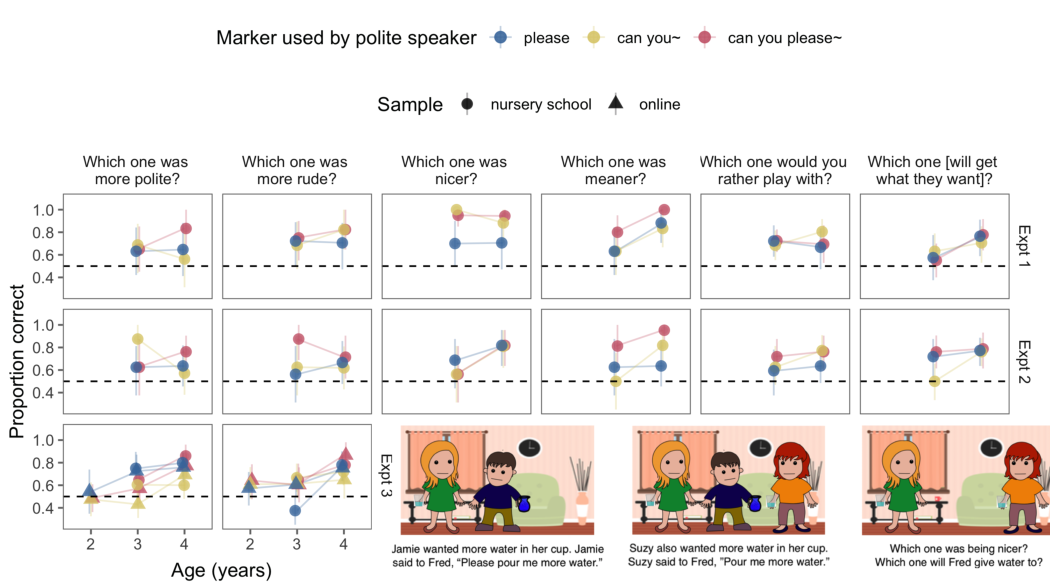
\includegraphics{figs/fig_results_placement-1} 

}

\caption[Bottom right]{Bottom right: Story example. Top, left: Results. Proportion of correct responses to questions comparing between a speaker who used a polite marker (where blue indicates "please", yellow "can you", and red "can you please") versus a speaker who did not. Data are binned into one-year age groups. Each row represents data from a different Experiment. Columns represent different questions asked. Dashed line represents chance level at 50\% (i.e., if participant were guessing at random).}\label{fig:fig_results_placement}
\end{figure*}
\end{CodeChunk}

We looked at the proportion of correct responses to various questions to
compare between a speaker who used a polite marker and spoke kindly,
versus a speaker who did not use a polite marker and spoke meanly
(Figure~\ref{fig:fig_results_placement}, first row). First, did children
understand that speakers who used polite markers are more polite and
nicer, and less rude and mean? Children struggled with the \emph{polite}
question (``Which one was more polite?'') as their average accuracy did
not differ from chance for almost all combinations of age and marker
types (all \(t>\).05 except for 4-year-olds' performance with ``can you
please'' marker). Children answered other questions more accurately but
depending on the marker type and age. For the \emph{nice} question, both
age groups gave accurate answers given ``can you'' and ``can you
please.'' For the \emph{rude} and \emph{mean} questions, children of
both ages answered correctly given ``can you please'' (all \(t<\).05)
but only 4-year-olds performed above chance given ``can you.''

Second, did children understand that speakers who spoke politely are
likely to be better play partners and to gain compliance from the
addressee? For the \emph{play partner} question, children from both age
groups successfully indicated the politely-speaking character as their
play partner choice for all three markers (except for 4-year-olds who
did not perform above chance given ``please''). For the
\emph{compliance} question, only 4-year-olds answered correctly given
all markers.

Interestingly, children overall struggled to give correct answers based
on the marker ``please''; only 4-year-olds successfully answered the
\emph{mean} and \emph{compliance} question but otherwise both age groups
failed to answer above chance given ``please.''

Third, did children show improvement with age for reasoning about polite
speech? As mentioned above, 4-year-olds answered most of the questions
accurately (except regarding ``please''), whereas 3-year-olds performed
above chance for just a few combinations of question types and markers.

A mixed-effects logistic regression predicting accuracy based on age,
question type and marker type\footnote{for Experiments 1 and 2, we use
  this model structure:
  \texttt{accuracy\ \textasciitilde{}\ age\ x\ question\ type\ x\ marker\ type\ +\ (1\ \textbar{}\ item)},
  where age is centered and scaled. All categorical variables were
  deviation coded, with specified contrasts of interest for the question
  type. Significance was calculated using the standard normal
  approximation to the \(t\) distribution (Barr, Levy, Scheepers, \&
  Tily, 2013).} confirmed there was an improvement with age (\(\beta\) =
0.2, \(p =\) 0.026). The regression model also confirmed that children
seemed to find some question types easier than others: Responses to
\emph{nice} and \emph{mean} questions were more accurate than to
\emph{polite} and \emph{rude} questions (\(\beta\) = 0.8, \(p =\)
0.002), whereas social implication questions (\emph{play partner} and
\emph{compliance}) were overall more difficult compared to speaker
attribute questions (\emph{polite}, \emph{rude}, \emph{nice}, and
\emph{mean}; \(\beta\) = -0.33, \(p =\) 0.006).

In sum, in this first experiment, we saw preliminary evidence that
children pay attention to and understand some cues to politeness and are
able to use these cues to infer whether speakers are relatively polite,
rude, nice or mean, and whether speakers are good play partners and are
likely to gain what they wanted from their addressees. 4-year-olds
answered questions accurately more often compared to 3-year-olds, but
both age groups tended to be accurate when all the possible cues were
used to signal that one speaker was polite (used ``can you
please\textasciitilde{}'', spoke with a kind tone and face) and the
other speaker wasn't (did not use a polite marker, spoke with an angry
tone and face).

However, one possible explanation for the finding in Experiment 1 is
that children are not using the linguistic polite markers (e.g.,
``please'') per se, and rather prosodic and facial cues that accompany
these markers. That is, children may have relied on the speaker's kind
voice and face rather than their use of ``please'' to evaluate their
niceness or likeability as a play partner. Similarly, greater accuracy
for some questions over others (e.g., ``nice'' \textgreater{}
``polite'') may have been due to greater association between some of the
words and prosodic and facial cues (e.g., a kind face may be seen to
signal niceness more than politeness), not due to greater understanding
for those words or concepts. Another potential concern is that the
experimenter was aware of the manipulations (i.e., they knew which
speaker was supposed to be ``polite'') and thus could have affected the
presentation of these speakers in ways that are not consistent across
all participants. In our next two experiments, we sought to address
these issue, and remove potentially confounding cues.

\section{Experiment 2}\label{experiment-2}

In Experiment 1, we saw initial evidence that children are able to use
some combinations of linguistic, prosodic, and facial cues to
politeness. In Experiment 2, we examined whether children are able to
make similar judgments using linguistic and prosodic cues only, without
facial expressions. For this, we used pre-recorded voiceovers to present
speaker utterances, so that (1) we could look at children's judgments
based on linguistic markers and prosodic cues only, and (2) we could
remove the role of potential bias of the experimenter in presentation of
these utterances.

\subsection{Methods}\label{methods-1}

\subsubsection{Participants}\label{participants-1}

3-year-old (\(n=\) 16; 8 F, \(M_{age}\) = 3.56 years, \(SD_{age}\) =
0.29) and 4-year-old children (\(n=\) 22; 13 F, \(M_{age}\) = 4.5 years,
\(SD_{age}\) = 0.32) were recruited from a local preschool. An
additional 5 children were tested but excluded due to failure on the
practice questions.

\subsubsection{Stimuli and design}\label{stimuli-and-design-1}

The design was identical to Experiment 1. Stimuli were the same as
Experiment 1 except two changes: (1) Instead of a picture book, we
presented the stories on a tablet; (2) the speakers' utterances were now
presented as recorded voiceovers. The voiceovers were recorded by native
English speakers, and contained prosodic cues that matched the
presence/absence of a polite marker (e.g., ``Please pour me more water''
was recorded with a kind voice and ``pour me more water'' with an angry
voice).

\subsubsection{Procedure}\label{procedure-1}

The procedure was identical to Experiment 1, except for the following
change: The participants now had to tap on a speaker on tablet in order
either to hear them speak, or to choose an answer to the questions
asked.

\subsection{Results and Discussion}\label{results-and-discussion-1}

Overall we saw similar patterns of results in Experiment 2 compared to 1
(Figure~\ref{fig:fig_results_placement}, second row). First, for
children's responses to speaker attribute questions, children still
struggled with the \emph{polite} question, with only 3-year-olds
answering above chance given ``can you'' and 4-year-olds given ``can you
please,'' but no other age group performing above chance given other
markers. For the \emph{rude} and \emph{mean} questions, similarly to
Experiment 1 results, children of both ages answered correctly given
``can you please'' (all \(t<\).05) but only 4-year-olds performed above
chance given ``can you.'' For the \emph{nice} question, unlike in
Experiment 1, 3-year-olds did not reach accuracy above chance for any of
the markers while 4-year-olds did answer accurately given all three
marker types.

Second, for children's responses to social implication questions,
results varied slightly: whereas both age groups were correct with the
\emph{play partner} question for most of the marker types for Experiment
1, 3- nd 4-year-olds were only accurate given ``can you please,'' and
only 4-year-olds answered accurately given ``can you.'' For the
\emph{compliance} question, however, the results shifted such that both
age groups answered accurately for all three markers, except for
3-year-olds not differing from chance level. Overall, again we saw
improvement with age for many of the combinations of question types and
markers.

A mixed-effects logistic regression predicting accuracy based on age,
question type and marker type confirmed that there was an effect of age
(\(\beta\) = 0.25, \(p =\) 0.002), and children made accurate judgments
more often when the marker used was ``can you please'' compared to
``please'' and ``can you'' together (\(\beta\) = 0.33, \(p =\) 0.019).
There was no main effect of question type, but there was an interaction
between age and question type such that performance for \emph{nice} and
\emph{mean} questions saw greater improvement with age than for
\emph{polite} and \emph{rude} questions (\(\beta\) = 0.57, \(p =\)
0.011).

In sum, across Experiments 1 and 2, we were able to confirm that
children are able to make accurate judgments about speakers given their
use of polite markers, especially ``can you please,'' and that as they
get older, children get better in their use of politeness cues to
respond to questions about speaker attributes and social implications.
Next, we wanted to see whether children are able to evaluate speakers
based on linguistic markers only, without any other supporting cues such
as prosodic cues or facial expressions.

\section{Experiment 3}\label{experiment-3}

\subsection{Methods}\label{methods-2}

\subsubsection{Participants}\label{participants-2}

We recruited two samples of participants: one from the same local
nursery school as Experiments 1 and 2, and the other from Lookit
(\url{https://lookit.mit.edu/}), an online platform for child research
participation, in which parents and their children can participate
together. The nursery school sample consisted of 3-year-old (\(n=\) 24;
11 F, \(M_{age}\) = 3.65 years, \(SD_{age}\) = 0.26) and 4-year-old
children (\(n=\) 25; 13 F, \(M_{age}\) = 4.48 years, \(SD_{age}\) =
0.28). An additional 3 children were tested but excluded due to failure
on the practice questions.

The online sample consisted of 2-year-old (\(n=\) 23; 12 F, \(M_{age}\)
= 2.48 years, \(SD_{age}\) = 0.29), 3-year-old (\(n=\) 31; 15 F,
\(M_{age}\) = 3.59 years, \(SD_{age}\) = 0.27) and 4-year-old children
(\(n=\) 27; 12 F, \(M_{age}\) = 4.46 years, \(SD_{age}\) = 0.29). An
additional 32 children were tested but excluded due to failure on the
practice questions (\(n=\) 19) or completion of fewer than half of the
test trials (\(n=\) 13).

\subsubsection{Stimuli}\label{stimuli}

For the nursery school sample, stimuli were identical to Experiment 2
except that the voiceovers for all utterances had the same prosody: All
utterances ended with a rising intonation. For the online sample,
stimuli were identical to what the nusery school participants saw except
that the story narration (other than speaker utterances) were also
pre-recorded such that parents did not need to read the stories aloud
themselves.

\subsubsection{Procedure}\label{procedure-2}

For the nursery school sample, the procedure was identical to Experiment
2. For the online sample, the procedure was similar except that parents
and children participated together at home and there was no experimenter
present. Parents accessed the webpage for the study and gave their
consent for participation, and then read instructions to proceed through
the different stories, which specified with an emphasis to not help
their children answer the questions.

\subsection{Results and Discussion}\label{results-and-discussion-2}

For Experiment 3, we were able to look at how children answered the
\emph{polite} and \emph{rude} questions given the same three marker
types as before, with three age groups including 2-year-olds. Because we
did not see any effect of sample in our mixed-effects logistic
regression model, we report on their performances averaged across the
two samples (though we do show the data separately in Figure
~\ref{fig:fig_results_placement}).

Unlike the two previous experimentss, 3- and 4-year-old children were
reliably accurate in their answers to both the \emph{polite} and
\emph{rude} questions (except 3-year-olds were not above chance for the
\emph{polite} question given ``can you'' and for the \emph{rude}
question given ``please''). Most strikingly, whereas children
consistently failed to answer these two questionss given the marker
``please,'' both age groups were clearly accurate on the \emph{polite}
question and 4-year-olds were accurate on the \emph{rude} question in
this current experiment.

A mixed-effects logistic regression\footnote{Model structure:
  \texttt{accuracy\ \textasciitilde{}\ sample\ +\ age\ x\ question\ type\ x\ marker\ type\ +\ (1\ \textbar{}\ item)}}
showed improvement with age (\(\beta\) = 0.19, \(p =\) 0.033) as well as
better performance for ``can you please'' than ``please'' and ``can
you'' together (\(\beta\) = 0.42, \(p =\) 0.002), consistent with
Experiment 2 results. Performance for ``please'' was also better than
for ``can you please'' and ``please'' together, confirming our
observation above: Children accurately compared between a speaker using
``please'' and another speaker not using it. One possible explanation is
that controlling for prosodic cues actually made it \emph{easier} to
compare between two utterances. Because we had stripped all the other
variations, it may have made the contrast between the presence and
absence of the marker ``please'' \emph{more} salient.

Additionally the regression model showed that children were better with
the \emph{polite} questions than \emph{rude} (\(\beta\) = -0.19, \(p =\)
0.04), and that responses to the \emph{polite} question given the marker
``please'' were more accurate than the \emph{rude} question given
``please'' (\(\beta\) = 0.42, \(p =\) 0.002). Finally, children showed a
greater improvement with age for ``can you please'' compared to
``please'' and ``can you'' together.

\section{General Discussion}\label{general-discussion}

What do young children understand about polite speech? In three
experiments, we looked at how 2- to 4-year-old children reason about
making requests with or without simple polite markers such as
``please'', ``can you'' and ``can you please.'' Our findings suggest
that by 3 years, children pay attention to the use of polite markers to
accurately judge whether that speaker is relatively more polite, rude,
nicer or meaner compared to another speaker. By 4 years, they are able
to reliably infer that a speaker who uses a polite marker is a better
play partner and is more likely to get what they wanted from the
addressee. Across all three experiments, we saw a clear developmental
trend such that children improved in their reasoning about polite speech
with increasing age.

Finally, though there were variations in children's performances across
the three experiments, there weren't consistent trends that indicated
having more cues to politeness is necessarily more helpful for children.
In fact, Experiment 3 with no facial or prosodic cues showed greatest
success by 3-year-olds to questions about who was more polite/rude,
which suggests that the presence of a polite marker is enough to signal
speaker attributes to children.

There are limitations to the current work that present opportunities for
future research. First, because this work looked only at the behaviors
of English-speaking children in the US, it is an open question how
children with different language and cultural background may develop
understanding of polite speech. Cross-cultural investigation of what
markers are present in other languages and cultures, as well as how
those markers are acquired, will be informative.

Second, we did not manipulate the statuses of speakers or addressees.
Though not explicitly stated, the visual depiction and narration used
for the current work suggested that speakers were communicating with
their peers only. However, =one key prediction from politeness theory is
that speakers will adjust their utterances based on the status of the
addressees (Brown \& Levinson, 1987). Indeed there is evidence that
children do adjust their speech based on the listener status and age:
Even at two years, children produce a polite form of request (e.g. ``Can
I have\ldots{}'') to an adult but an imperative form (e.g. ``Give
me\ldots{}'') to a peer (Corsaro, 1979; Shatz \& Gelman, 1973); Children
around 2.5 years were to found to use less polite language with their
fathers compared to their mothers (Ervin-Tripp, Guo, \& Lampert, 1990).
Wagner, Greene-Havas, \& Gillespie (2010) showed that by 4 years,
children understand that formal speech (``Excuse me please, can you tell
me your name?'') is addressed toward a figure of authority (e.g., a
teacher rather than a little girl), but it is yet unclear what cues
(linguistic markers, social cues) in formal speech children are using to
make such prediction (Wagner, Vega-Mendoza, \& Van Horn, 2014). Thus,
future work should examine how children use cues to politeness to judge
speaker intentions in different contexts, including varied status
differences between speakers and listeners.

In sum, the current work showed that young children understand
implications of using simple polite markers in requests. These findings
fill the gap in literature about how children reason about polite
speech, and pragmatics in general.

\section{References}\label{references}

\setlength{\parindent}{-0.1in} \setlength{\leftskip}{0.125in} \noindent

\hypertarget{refs}{}
\hypertarget{ref-barr2013}{}
Barr, D. J., Levy, R., Scheepers, C., \& Tily, H. J. (2013). Random
effects structure for confirmatory hypothesis testing: Keep it maximal.
\emph{Journal of Memory and Language}, \emph{68}(3), 255--278.

\hypertarget{ref-bates1976}{}
Bates, E. (1976). Acquisition of polite forms: Experimental evidence.
\emph{Language and Context: The Acquisition of Pragmatics}, 295--326.

\hypertarget{ref-bates1977}{}
Bates, E., \& Silvern, L. (1977). Social adjustment and politeness in
preschoolers. \emph{Journal of Communication}, \emph{27}(2), 104--111.

\hypertarget{ref-bock1981}{}
Bock, J. K., \& Hornsby, M. E. (1981). The development of directives:
How children ask and tell. \emph{Journal of Child Language},
\emph{8}(01), 151--163.

\hypertarget{ref-bonnefon2011}{}
Bonnefon, J.-F., Feeney, A., \& De Neys, W. (2011). The risk of polite
misunderstandings. \emph{Current Directions in Psychological Science},
\emph{20}(5), 321--324.

\hypertarget{ref-brown1987}{}
Brown, P., \& Levinson, S. C. (1987). \emph{Politeness: Some universals
in language usage} (Vol. 4). Cambridge university press.

\hypertarget{ref-buhler1934}{}
Buhler, K. (1934). \emph{Sprachtheorie}. Oxford, England: Fischer.

\hypertarget{ref-clark1980}{}
Clark, H. H., \& Schunk, D. H. (1980). Polite responses to polite
requests. \emph{Cognition}, \emph{8}(2), 111--143.

\hypertarget{ref-corsaro1979}{}
Corsaro, W. A. (1979). Young children's conception of status and role.
\emph{Sociology of Education}, 46--59.

\hypertarget{ref-ervin1982}{}
Ervin-Tripp, S. M. (1982). Ask and it shall be given unto you:
Children's requests. \emph{Georgetown University Roundtable on Languages
and Linguistics. Contemporary Perceptions of Language: Interdisciplinary
Dimensions}, 235--245.

\hypertarget{ref-ervin1990}{}
Ervin-Tripp, S. M., Guo, J., \& Lampert, M. (1990). Politeness and
persuasion in children's control acts. \emph{Journal of Pragmatics},
\emph{14}(2), 307--331.

\hypertarget{ref-goodman2013}{}
Goodman, N. D., \& Stuhlmuller, A. (2013). Knowledge and implicature:
Modeling language understanding as social cognition. \emph{Topics in
Cognitive Science}, \emph{5}(1), 173--184.

\hypertarget{ref-holtgraves1997}{}
Holtgraves, T. (1997). YES, but... positive politeness in conversation
arguments. \emph{Journal of Language and Social Psychology},
\emph{16}(2), 222--239.

\hypertarget{ref-ide1989}{}
Ide, S. (1989). Formal forms and discernment: Two neglected aspects of
universals of linguistic politeness. \emph{Multilingua-Journal of
Cross-Cultural and Interlanguage Communication}, \emph{8}(2-3),
223--248.

\hypertarget{ref-jakobson1960}{}
Jakobson, R. (1960). Linguistics and poetics. In \emph{Style in
language} (pp. 350--377). MA: MIT Press.

\hypertarget{ref-leech1983}{}
Leech, G. (1983). \emph{Principles of pragmatics}. London, New York:
Longman Group Ltd.

\hypertarget{ref-nippold1982}{}
Nippold, M. A., Leonard, L. B., \& Anastopoulos, A. (1982). Development
in the use and understanding of polite forms in children. \emph{Journal
of Speech, Language, and Hearing Research}, \emph{25}(2), 193--202.

\hypertarget{ref-read1978}{}
Read, B. K., \& Cherry, L. J. (1978). Preschool children's production of
directive forms. \emph{Discourse Processes}, \emph{1}(3), 233--245.

\hypertarget{ref-shannon1948}{}
Shannon, C. E. (1948). A mathematical theory of communication.
\emph{Bell Syst. Tech. J.}, \emph{27}, 623--656.

\hypertarget{ref-shatz1973}{}
Shatz, M., \& Gelman, R. (1973). The development of communication
skills: Modifications in the speech of young children as a function of
listener. \emph{Monographs of the Society for Research in Child
Development}, 1--38.

\hypertarget{ref-wagner2010}{}
Wagner, L., Greene-Havas, M., \& Gillespie, R. (2010). Development in
children?s comprehension of linguistic register. \emph{Child
Development}, \emph{81}(6), 1678--1686.

\hypertarget{ref-wagner2014}{}
Wagner, L., Vega-Mendoza, M., \& Van Horn, S. (2014). Social and
linguistic cues facilitate children?s register comprehension.
\emph{First Language}, \emph{34}(4), 299--314.

\hypertarget{ref-yoon2017}{}
Yoon, E. J., Tessler, M. H., Goodman, N. D., \& Frank, M. C. (2017). ``I
won't lie, it wasn't amazing": Modeling polite indirect speech. In
\emph{Proceedings of the thirty-ninth annual conference of the Cognitive
Science Society}.

\bibliographystyle{apacite}


\end{document}
